\documentclass{beamer}

%\usetheme[framenumber,totalframenumber]{UniversiteitGent}
%\usetheme[faculty=di,framenumber,totalframenumber]{UniversiteitGent}
%\usetheme[faculty=we,usecolors,framenumber,totalframenumber]{UniversiteitGent}
%\usetheme[language=english,framenumber,totalframenumber]{AlleghenyCollege}
\usetheme{AnnArbor}
\usecolortheme{dove}

\title{CMPSC 390 \\ Bitcoin Interactions}
\author{Janyl Jumadinova}
\date{February 1, 2021}

\long\def\omitit#1{}

\usepackage{hyperref}
\hypersetup{
    colorlinks=true,
    linkcolor=blue,
    filecolor=magenta,      
    urlcolor=cyan,
}

\begin{document}

\begin{frame}
  \titlepage
\end{frame}

%%%%%%%%%%%% Slide %%%%%%%%%%%%%%%%%%%%%%%%%%%%%%%%%%%%%%%%%%%%%%%%%%%
\begin{frame}
  \frametitle{Light Nodes (SPV Nodes) }
 	\begin{block}{\textcolor{brown}{Simple Payment Verification (SPV): }}
 	 a method for verifying if particular transactions are included in a block without downloading the entire block.
 	\end{block}
 	\pause
 	\centering
	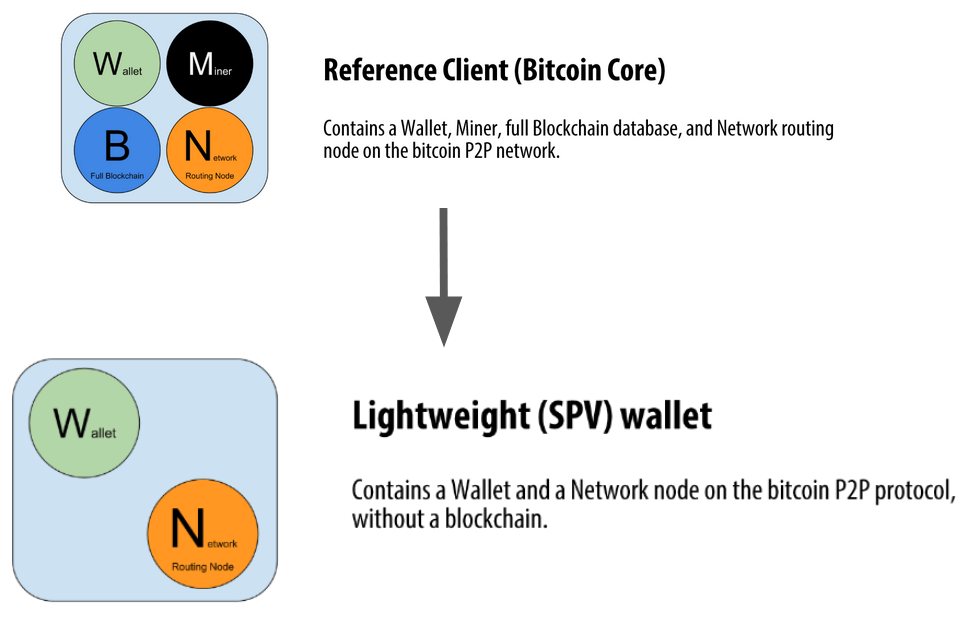
\includegraphics[scale=0.35]{nodes}
\end{frame}
%%%%%%%%%%%% Slide %%%%%%%%%%%%%%%%%%%%%%%%%%%%%%%%%%%%%%%%%%%%%%%%%%%
\begin{frame}
  \frametitle{Simple Payment Verification}
 	\begin{block}{\textbf{Assumption}: }
Incoming block headers are not from a false chain.
 	\end{block}
 	\centering
	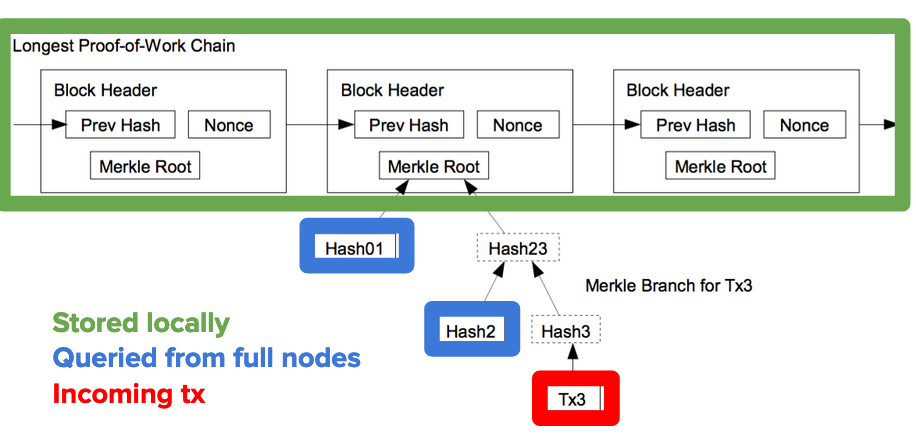
\includegraphics[scale=0.5]{transact}
\end{frame}

%%%%%%%%%%%% Slide %%%%%%%%%%%%%%%%%%%%%%%%%%%%%%%%%%%%%%%%%%%%%%%%%%%
\begin{frame}
  \frametitle{Bitcoin Wallets}
  \pause
  \begin{itemize}
  	\item Provides a user interface to the blockchain
	\item Keep track of the private key
	\item Store, send, receive, and list transactions
	\item Maybe some other  functionalities

  \end{itemize}
  $ $ \\ 
  \pause
  \url{https://bitcoin.org/en/choose-your-wallet}
\end{frame}
%%%%%%%%%%%% Slide %%%%%%%%%%%%%%%%%%%%%%%%%%%%%%%%%%%%%%%%%%%%%%%%%%%
\begin{frame}
  \frametitle{Types of Wallets}
 	\centering
	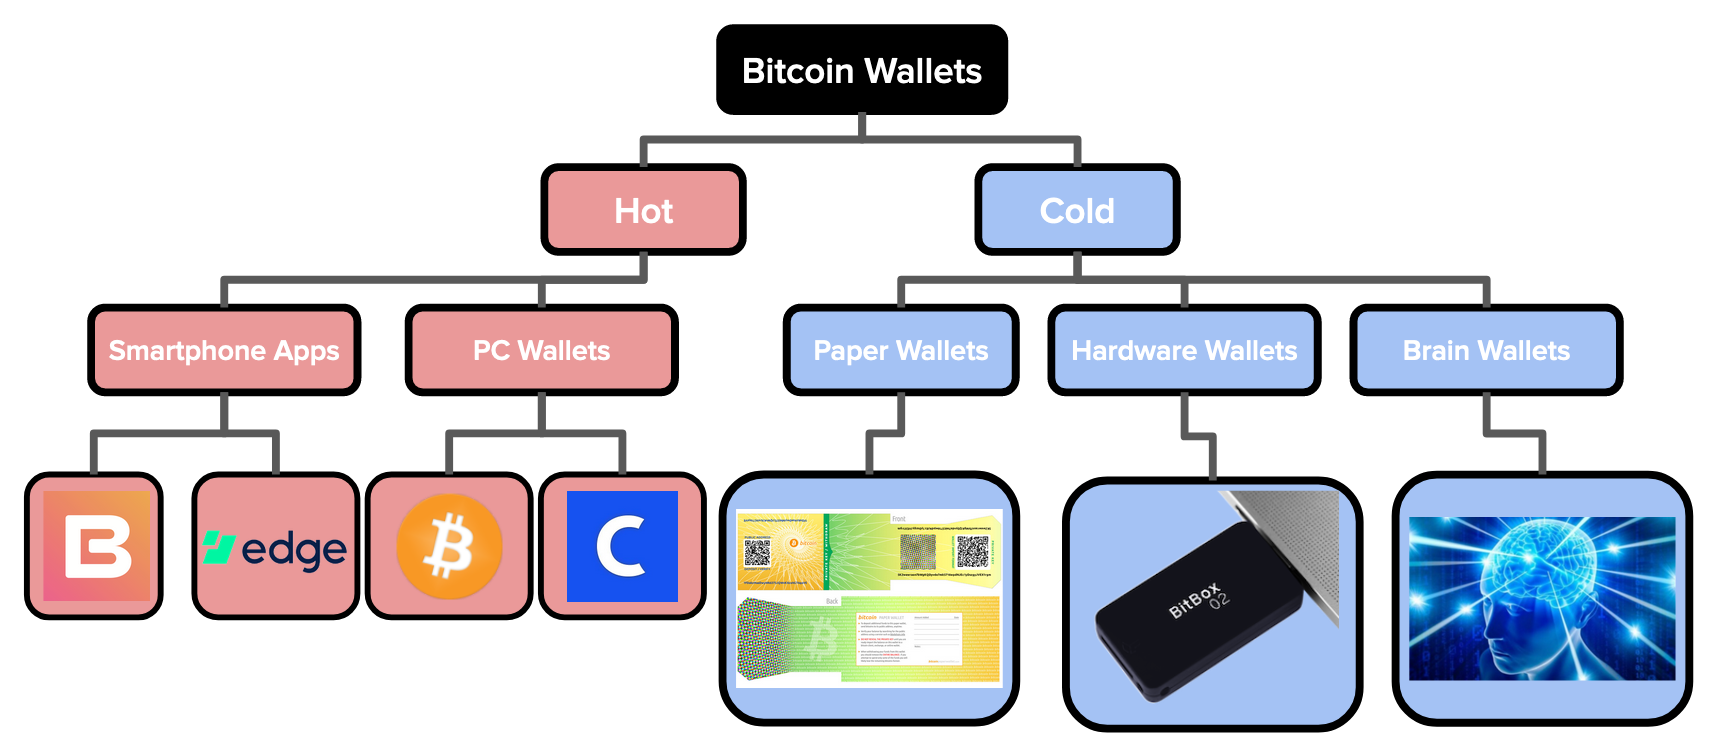
\includegraphics[scale=0.4]{wallets}
\end{frame}
%%%%%%%%%%%% Slide %%%%%%%%%%%%%%%%%%%%%%%%%%%%%%%%%%%%%%%%%%%%%%%%%%%
\begin{frame}
  \frametitle{Creating a Wallet}
  
	\begin{itemize}
		\item Paper/hardware  wallet (example: \url{https://walletgenerator.net/})
		\item Digital wallet (example: \url{https://login.blockchain.com/\#/signup})
	\end{itemize}
\end{frame}
%%%%%%%%%%%% Slide %%%%%%%%%%%%%%%%%%%%%%%%%%%%%%%%%%%%%%%%%%%%%%%%%%%
\begin{frame}
  \frametitle{Getting bitcoin}
  	\begin{itemize}
  		\item Bitcoin ATMs (\url{https://coinucopia.io/}) \pause
  		\item Centralized Exchanges (\url{https://bitcoin.org/en/exchanges}) \pause
  		\item Decentralized Exchanges (DEXs) (example: \url{https://bisq.network/})
  	\end{itemize}
\end{frame}

%%%%%%%%%%%% Slide %%%%%%%%%%%%%%%%%%%%%%%%%%%%%%%%%%%%%%%%%%%%%%%%%%%
\begin{frame}
  \frametitle{Best Practices}
  
\begin{itemize}
	\item Multisignature
	\item Never reuse pseudonyms, public keys
	\begin{itemize}
		\item Wallet software can handle this
	\end{itemize}
\end{itemize}
\end{frame}
%%%%%%%%%%%% Slide %%%%%%%%%%%%%%%%%%%%%%%%%%%%%%%%%%%%%%%%%%%%%%%%%%%
\begin{frame}
  \frametitle{Hierarchical Deterministic (HD) Wallets}
	\begin{itemize}
		\item Deterministic because all child keys are generated from a seed in the same way every time.
		\item \textbf{Hierarchical}: you can organize the keys in a tree-like structure, with levels.
	\end{itemize}
	\centering
	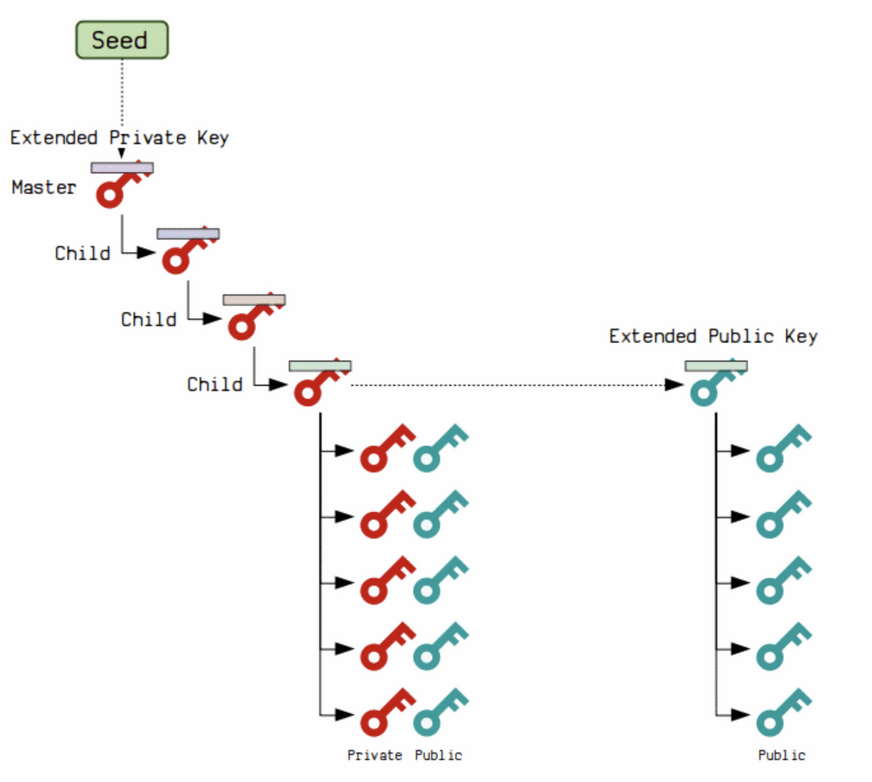
\includegraphics[scale=0.42]{hd}
\end{frame}

%%%%%%%%%%%% Slide %%%%%%%%%%%%%%%%%%%%%%%%%%%%%%%%%%%%%%%%%%%%%%%%%%%
\end{document}
